\documentclass[sigconf,review,anonymous]{acmart}

\usepackage{tikz}
\usetikzlibrary{arrows.meta,backgrounds,fit,positioning}
\usepackage{placeins}
\usepackage{xspace}
\usepackage{seqsplit}

\definecolor{CARRorange}{RGB}{207,96,35}
\definecolor{FrozenBlue}{RGB}{43,92,135}
\definecolor{MemoryPurple}{RGB}{103,78,134}

% DAI 2026 Research Track review version: ACM sigconf, two-column, anonymous.
% Replace the review metadata below only after acceptance and receipt of the
% official ACM eRights/TAPS metadata.
\AtBeginDocument{%
  \providecommand\BibTeX{{%
    Bib\TeX}}}
\setcopyright{none}
\acmYear{2026}
\acmConference[DAI 2026]
  {The 8th International Conference on Distributed Artificial Intelligence}
  {November 29--December 2, 2026}
  {Hong Kong, China}
% The DAI 2026 CFP does not currently require an ID in the PDF. Enable only if
% the program chairs explicitly request it:
% \acmSubmissionID{<OpenReview submission number>}

\newcommand{\carr}{\textsc{CARR}\xspace}
\newcommand{\norecall}{\textsc{CARR-NoRecall}\xspace}
\newcommand{\bbootstrap}{\textsc{Bootstrap}\xspace}
\newcommand{\exactfour}{\textsc{Exact-G4}\xspace}
\newcommand{\exactfive}{\textsc{Exact-G5}\xspace}
\newcommand{\randomfive}{\textsc{Random-G5}\xspace}
\newcommand{\jsfive}{\textsc{JS-G5}\xspace}
\newcommand{\exactdense}{\textsc{Exact-B25}\xspace}

\graphicspath{{figures/}}

\begin{document}

\title[When Should Global Guidance Be Refreshed?]
  {When Should Global Guidance Be Refreshed? A Paired Pareto Study in Lifelong Multi-Agent Path Finding}

\author{Anonymous Author(s)}
\renewcommand{\shortauthors}{Anonymous Author(s)}

\begin{abstract}
Lifelong multi-agent path finding (LMAPF) requires robot fleets to serve an
ongoing stream of goals while avoiding congestion. Learned global guidance can
improve traffic flow, but existing online methods commonly refresh guidance at
fixed intervals. Frequent refresh consumes generator calls even when demand is
stable, whereas infrequent refresh may leave guidance stale after workload
shifts. We formulate refresh timing as a budgeted control problem and
introduce Context-Aware Refresh and Recall (\carr), which causally chooses to
retain active guidance, generate a new graph, or reactivate a previously
generated one using demand change, context similarity, guidance age, and
route-adoption signals. \carr wraps a frozen generator and planner without
retraining either. We evaluate eight refresh policies on stationary and
non-stationary warehouse workloads using
paired, policy-independent task streams and an audit-complete protocol.
The pre-specified primary objective is not met: dense refresh retains a small
but measurable mean-throughput advantage (\carr effect $-0.80\%$; 95\% CI
$[-1.19\%,-0.40\%]$), so 1\% non-inferiority is not established. In
pre-specified secondary analyses, \carr uses about 79\% fewer generator calls,
forms a non-dominated sample-mean throughput--call operating point, and
significantly outperforms all five evaluated low-call comparators. Our results
identify guidance timing as an independent systems-design dimension and
provide a reproducible basis for choosing refresh policies according to
resource constraints.
\end{abstract}

\keywords{lifelong multi-agent path finding, multi-robot coordination,
adaptive global guidance, resource-aware planning, event-triggered refresh,
non-stationary workloads, Pareto analysis}

\ccsdesc[500]{Computing methodologies~Multi-agent systems}
\ccsdesc[300]{Computing methodologies~Motion path planning}

\maketitle

\section{Introduction}

Lifelong multi-agent path finding (LMAPF) asks a fleet of agents to serve an
ongoing stream of goals without collisions while maintaining throughput
\cite{ma2017lifelong}. Scalable solvers often separate a shared, slowly varying
coordination signal from fast local motion decisions. Direction maps,
highways, guide paths, and learned guidance graphs all bias agents away from
congested interactions \cite{jansen2008direction,cohen2015highways,
chen2024traffic,ijcai2024p0035}. OnlineGGO advances this idea by conditioning
guidance on recent traffic and task distributions, but its update interval
still controls a stated trade-off between adaptability and recomputation
\cite{zang2025online}.

This leaves an orthogonal control-plane question: \emph{given a fixed guidance
generator and planner, when is another generator invocation warranted?}
Periodic refresh ignores whether demand has changed. Refreshing at every
opportunity consumes calls even when the active artifact remains appropriate;
refreshing rarely can retain stale traffic preferences after a workload
shift. A previous graph may also become relevant again when demand recurs.
The resulting decision is not simply whether guidance is useful, but how much
throughput each additional invocation buys.

We study this question in a frozen OnlineGGO-style CNN+GPIBT system. Our
controller, Context-Aware Refresh and Recall (\carr), chooses among holding the
active graph, generating a new graph, and reinstalling a historical graph.
It observes only causally available endpoint histograms, event history,
guidance age, and route-adoption maturity. The generator, downstream planner,
simulator, and evaluation task tapes are identical for every policy. We ask:

\begin{itemize}
  \item \textbf{RQ1:} Does context-aware refresh improve throughput over no
  online refresh and weak sparse schedules?
  \item \textbf{RQ2:} What throughput--call trade-off does it achieve relative
  to dense periodic refresh?
  \item \textbf{RQ3:} Does historical reactivation add throughput or primarily
  substitute for fresh generations?
\end{itemize}

Our contributions are threefold. First, we formulate guidance publication as
a budgeted, causal control problem and instantiate \carr with explicit
generation, installation, and delayed-adoption semantics. Second, we provide a
fresh-root, paired evaluation of eight publication policies: 3{,}840 isolated
runs over forty independent root clusters, externally fixed task tapes,
root-cluster inference, multiplicity control, and an auditable no-deletion
ledger. Third, we report the failed primary non-inferiority result together
with its pre-specified secondary trade-off analyses. \carr uses 5.46 calls on
average, lies on the empirical sample-mean Pareto frontier, and significantly
outperforms all five frozen low-call comparators after correction; historical
recall shows no detected throughput benefit. We therefore make a bounded
resource--throughput claim within one frozen backbone, not a global LMAPF
state-of-the-art claim.

Figure~\ref{fig:carr-framework} separates the frozen LMAPF data plane from
\carr's sole intervention: a causal, budgeted decision over guidance
publication. This separation is central to our attribution claim. Any change
in a paired rollout must arise from which already-defined guidance operation
is executed, rather than from retraining the generator, modifying GPIBT, or
changing the exogenous task stream.

\begin{figure*}[t]
\centering
\resizebox{\textwidth}{!}{% Paper-native vector overview of the evaluated CARR control loop.
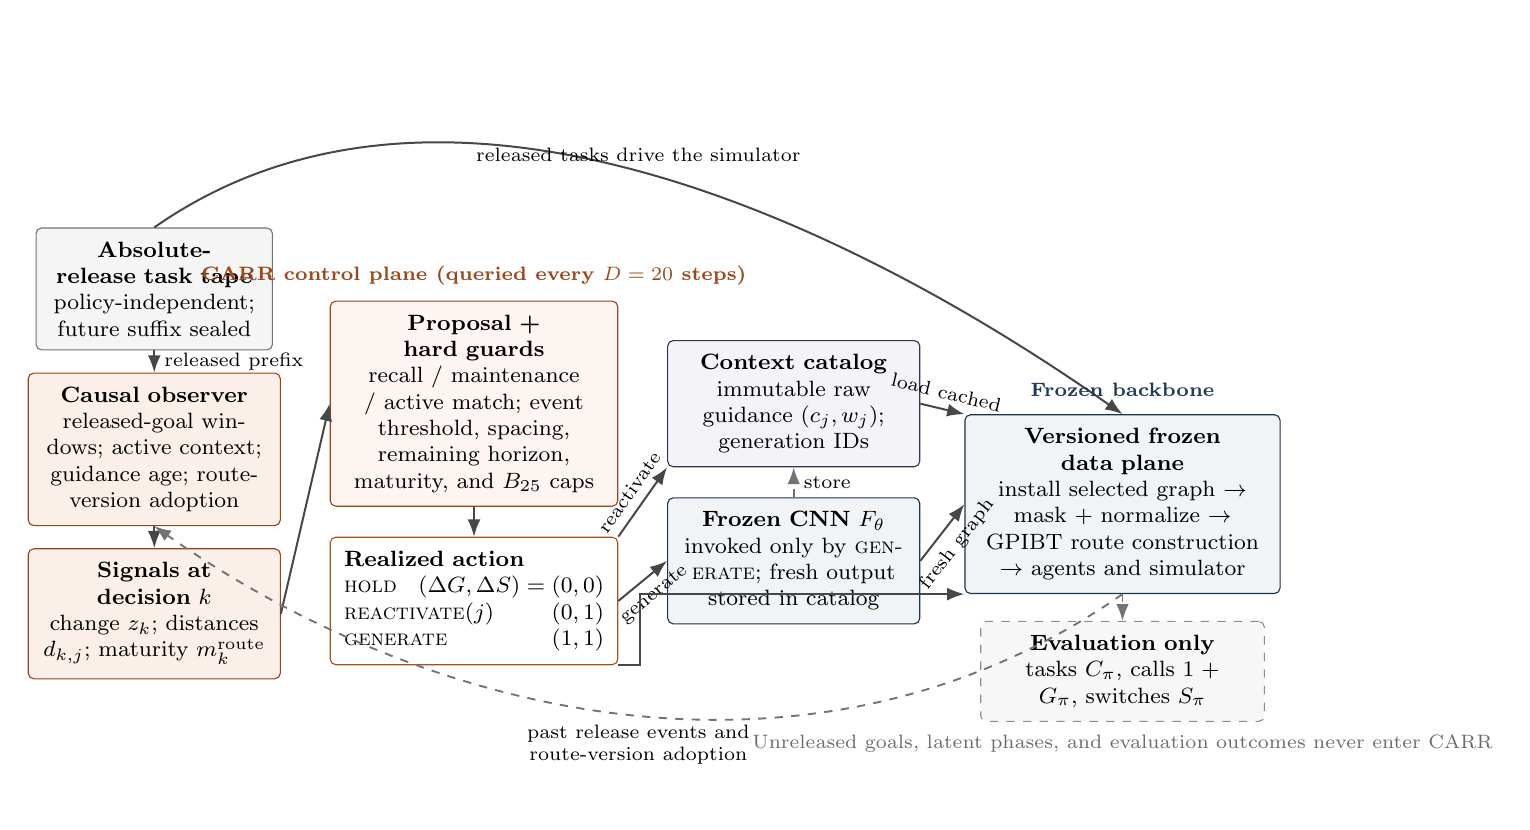
\begin{tikzpicture}[
  font=\footnotesize,
  >=Latex,
  flow/.style={->, line width=0.72pt, draw=black!72},
  feedback/.style={->, line width=0.68pt, draw=black!55, dashed},
  box/.style={draw=black!55, rounded corners=2pt, align=center,
              inner xsep=5pt, inner ysep=5pt, minimum height=1.08cm},
  exogenous/.style={box, fill=black!4, text width=2.65cm},
  carr/.style={box, fill=CARRorange!10, draw=CARRorange!72!black,
               text width=2.85cm},
  decision/.style={box, fill=CARRorange!6, draw=CARRorange!72!black,
                   text width=3.30cm},
  actions/.style={box, fill=white, draw=CARRorange!82!black,
                  text width=3.30cm, align=left},
  memory/.style={box, fill=MemoryPurple!7, draw=MemoryPurple!60!black,
                 text width=2.85cm},
  frozen/.style={box, fill=FrozenBlue!7, draw=FrozenBlue!58!black,
                 text width=2.85cm},
  dataplane/.style={box, fill=FrozenBlue!7, draw=FrozenBlue!58!black,
                    text width=3.65cm, minimum height=1.55cm},
  eval/.style={box, fill=black!3, draw=black!45, dashed,
               text width=3.25cm, minimum height=0.68cm}
]

% Exogenous and causal-observation stack.
\node[exogenous] (tape)
  {\textbf{Absolute-release task tape}\\policy-independent; future suffix sealed};
\node[carr, below=0.28cm of tape] (observer)
  {\textbf{Causal observer}\\released-goal windows; active context; guidance age; route-version adoption};
\node[carr, below=0.28cm of observer] (signals)
  {\textbf{Signals at decision $k$}\\change $z_k$; distances $d_{k,j}$; maturity $m_k^{\rm route}$};

% CARR decision stack.
\node[decision, right=0.62cm of observer, yshift=0.58cm] (guards)
  {\textbf{Proposal + hard guards}\\recall / maintenance / active match; event threshold, spacing, remaining horizon, maturity, and $B_{25}$ caps};
\node[actions, below=0.38cm of guards] (actions)
  {\textbf{Realized action}\\
   \textsc{hold}\hfill $(\Delta G,\Delta S)=(0,0)$\\
   \textsc{reactivate}$(j)$\hfill $(0,1)$\\
   \textsc{generate}\hfill $(1,1)$};

% Guidance sources and frozen data plane.
\node[memory, right=0.62cm of guards] (catalog)
  {\textbf{Context catalog}\\immutable raw guidance $(c_j,w_j)$; generation IDs};
\node[frozen, below=0.38cm of catalog] (cnn)
  {\textbf{Frozen CNN} $F_\theta$\\invoked only by \textsc{generate}; fresh output stored in catalog};
\node[dataplane, right=0.56cm of cnn, yshift=0.72cm] (dataplane)
  {\textbf{Versioned frozen data plane}\\install selected graph $\rightarrow$ mask + normalize $\rightarrow$ GPIBT route construction $\rightarrow$ agents and simulator};
\node[eval, below=0.34cm of dataplane] (evaluator)
  {\textbf{Evaluation only}\\tasks $C_\pi$, calls $1+G_\pi$, switches $S_\pi$};

% Main causal path.
\draw[flow] (tape) -- node[right, font=\scriptsize] {released prefix} (observer);
\draw[flow] (observer) -- (signals);
\draw[flow] (signals.east) -- (guards.west);
\draw[flow] (guards) -- (actions);

% Action semantics.  Branches stay in separate vertical bands.
\draw[flow] (actions.north east) -- node[above, sloped, font=\scriptsize] {reactivate} (catalog.south west);
\draw[flow] (actions.east) -- node[below, sloped, font=\scriptsize] {generate} (cnn.west);
\draw[flow] (actions.south east) -- ++(0.28,0) |- (dataplane.south west);
\draw[flow] (catalog.east) -- node[above, sloped, font=\scriptsize] {load cached} (dataplane.north west);
\draw[flow] (cnn.east) -- node[below, sloped, font=\scriptsize] {fresh graph} (dataplane.west);
\draw[feedback] (cnn.north) -- node[right, font=\scriptsize] {store} (catalog.south);

% Environment and evaluation flows are visually distinct.
\draw[flow] (tape.north) to[out=35,in=145,looseness=0.90]
  node[above, font=\scriptsize] {released tasks drive the simulator} (dataplane.north);
\draw[feedback] (dataplane.south) to[out=215,in=325,looseness=0.95]
  node[below, align=center, font=\scriptsize] {past release events and\\route-version adoption} (observer.south);
\draw[feedback] (dataplane) -- (evaluator);

\node[font=\scriptsize\bfseries, text=CARRorange!75!black,
      above=0.07cm of guards.north] {CARR control plane (queried every $D=20$ steps)};
\node[font=\scriptsize\bfseries, text=FrozenBlue!65!black,
      above=0.10cm of dataplane.north] {Frozen backbone};
\node[font=\scriptsize, text=black!58, below=0.04cm of evaluator.south]
  {Unreleased goals, latent phases, and evaluation outcomes never enter CARR};

\end{tikzpicture}
}
\caption{CARR's causal control plane around a frozen guidance generator,
GPIBT planner, and simulator. Past release and route-adoption events produce
the change, context, age, and maturity signals used to hold, reactivate, or
generate guidance under hard guards. Recall loads an immutable catalog entry
without invoking the CNN; generation calls the CNN and stores a new entry.
Installed versions reach agents only at route construction, and evaluation
outcomes do not feed back to the controller.}
\Description{System diagram showing a policy-independent task tape feeding a
causal CARR observer. Change, context, age, and route-adoption signals pass
through proposal and budget guards to hold, reactivate, or generate actions.
Reactivation loads a cached graph, generation invokes a frozen CNN, and both
feed a versioned installation used by a frozen GPIBT planner and simulator.
Only past task-release and route-adoption events return to the controller;
throughput and resource counts flow only to evaluation.}
\label{fig:carr-framework}
\end{figure*}

\section{Related Work}

\subsection{Lifelong multi-agent planning}

Early formulations of lifelong or online multi-agent routing include
pickup-and-delivery task streams and token-passing coordination
\cite{ma2017lifelong}. PIBT instead constructs agents' next actions using
priority inheritance and backtracking, with finite-time guarantees under
specific graph conditions \cite{ijcai2019p76}. RHCR repeatedly solves
bounded-horizon MAPF instances and represents a complementary replanning-based
family \cite{li2021rhcr}. We do not empirically compare these algorithm
families. Our study fixes a GPIBT-style downstream planner so that differences
can be attributed to guidance publication policy.

\subsection{Global traffic guidance}

Shared directional preferences have progressed from learned direction maps
and user-specified highways \cite{jansen2008direction,cohen2015highways} to
congestion-avoiding guide paths \cite{chen2024traffic}. Guidance Graph
Optimization (GGO) directly optimizes edge weights or a model that produces
them \cite{ijcai2024p0035}; later work extends the representation to mixed edge
directions and weights \cite{zhang2026mixed}. OnlineGGO dynamically generates
guidance from recent traffic and current task distributions and integrates it
with both direct and guide-path planning \cite{zang2025online}. These works
primarily ask what guidance should contain. We keep the learned generator
fixed and ask when its output should be retained, regenerated, or recalled.

\subsection{Adaptive update timing}

Update timing is an established control variable outside LMAPF. Event-triggered
control replaces strictly periodic execution with state-dependent events
\cite{tabuada2007event}; navigation work has studied learned replanning timing
and path-regeneration decisions in dynamic environments
\cite{honda2024when,han2018path}. We borrow the resource-aware motivation, not
their stability or navigation guarantees. Our setting differs in that a shared
guidance artifact influences many agents, adoption is delayed until route
construction, and evidence is evaluated as a paired throughput--call frontier.

\section{Problem Setting and System Semantics}

\subsection{Lifelong routing with fixed guidance generation}

Let $G=(V,E)$ be a directed grid graph and let $n$ agents repeatedly receive
sequential goal-reaching tasks. At each simulator step an agent waits or moves
to an adjacent vertex; vertex conflicts and opposing edge swaps are forbidden.
The planner consults a shared directed-edge guidance tensor while constructing
routes.

A frozen convolutional generator $F_\theta$ maps the causal traffic
observation at decision $k$ to a four-channel raw edge-weight tensor,
\begin{equation}
  w_k=F_\theta(o_{\leq t_k})\in\mathbb{R}^{4\times H_m\times W_m}.
\end{equation}
The environment masks invalid edges and normalizes $w_k$ before the GPIBT
backend consumes it. We vary only the policy that decides whether to hold,
replace, or recall guidance. The checkpoint, planner, simulator, maps, and task
tapes remain fixed.

Each episode contains a 200-step warm-up and a scored horizon of 2,000 steps.
Guidance decisions occur every $D=20$ steps, producing $N=100$ scored windows.
All policies make one mandatory bootstrap call. Of the 99 post-bootstrap
decisions, the focal ceiling is
\begin{equation}
  B_{25}=\lceil0.25(99)\rceil=25.
\end{equation}
For policy $\pi$, let $C_\pi$ be scored task completions, $G_\pi$ fresh
post-bootstrap generator calls, and $S_\pi$ effective post-bootstrap guidance
installations. We study the two-dimensional operating point
$(\mathbb{E}[1+G_\pi],\mathbb{E}[C_\pi])$ and report installations separately.
Generator calls are a pre-specified logical resource unit; they are not a proxy
for a measured wall-clock, energy, or monetary reduction.

\subsection{Publication-control objective}

At decision $k$, a publication controller has a causal history
$\mathcal{H}_k$ containing only observations exposed by time $t_k$, an active
generation, and (for memory policies) a catalog of earlier generations. It
maps this state to one of three operations. Define the per-decision resource
indicators
\begin{equation}
 g_k=\mathbb{1}[a_k=\textsc{generate}],\qquad
 s_k=\mathbb{1}[a_k\neq\textsc{hold}].
\end{equation}
The two counts are deliberately distinct. Generating installs a new artifact
and therefore increments both; reactivation installs an old artifact and
increments only $s_k$; holding increments neither. Excluding the mandatory
bootstrap, the focal policy obeys
\begin{equation}
 \sum_{k=1}^{N-1}g_k\leq B_{25},\qquad
 \sum_{k=1}^{N-1}s_k\leq B_{25}.
\end{equation}

We do not collapse throughput and calls into a hand-selected scalar reward.
Such a scalar would make the conclusion depend on an unmeasured conversion
between one generator invocation and one completed task. Instead, the primary
analysis separately tests throughput preservation against the dense reference,
and the secondary analysis exposes the empirical operating points in
call--throughput space. Policy $A$ point-dominates policy $B$ only when its
sample-mean call count is no larger and its sample-mean completion count is no
smaller, with at least one strict inequality. This descriptive frontier is
kept separate from inferential pairwise claims.

\subsection{Policy-independent task tapes}

Completion-driven task generation can confound a throughput comparison: a
faster policy advances its task random-number stream sooner and may receive a
different future workload. We instead materialize complete absolute-release
task tapes before timestep zero. For agent $i$,
\begin{equation}
  \mathcal{T}_i=((g_{i,0},r_{i,0}),\ldots,(g_{i,L_i-1},r_{i,L_i-1})),
\end{equation}
where $g_{i,j}$ is a goal and $r_{i,j}$ its absolute release time. Starts,
goals, releases, and identifiers are identical across paired policies and are
verified by independent fingerprints. We evaluate stationary, abrupt, and
recurrent endpoint distributions; recurrent demand follows an
$A\!\rightarrow\!B\!\rightarrow\!A\!\rightarrow\!B$ sequence. Phase metadata
and unreleased tape suffixes are never controller inputs.

The tape generator staggers each agent's releases over a common 110-step
interval, rather than releasing the whole fleet in a synchronized burst. A
stationary tape uses one endpoint-centered distribution throughout. Dynamic
tapes change the distribution at scored timesteps 500, 1,000, and 1,500. For
the abrupt workload, four distinct endpoint centers are selected
deterministically from the root, with adjacent distributions required to have
Jensen--Shannon separation of at least 0.30. For the recurrent workload, two
such centers alternate as $A\!\rightarrow\!B\!\rightarrow\!A\!\rightarrow\!B$.
Goals are then sampled once with root-keyed per-agent randomness and sealed
into the tape. Consequently, policies may complete different prefixes by the
horizon, but they cannot receive different goals merely because one policy
finishes earlier. A non-scoring guard suffix ensures that no arm exhausts its
finite tape during the measured horizon.

This construction also makes the information boundary testable. At decision
$k$, the controller sees trace events already released by $t_k$ and the
currently active goals. It does not see the registered workload label, the
locations of future phase changes, the selected phase centers, or any
unreleased goal. Metamorphic preflight checks altered future suffixes while
holding the observable prefix fixed and required the earlier controller trace
to remain unchanged.

\subsection{Generation, installation, and delayed adoption}

A \emph{generation ID} names one immutable output of $F_\theta$. An
\emph{installation version} increments whenever a fresh or historical graph
becomes active. Reactivating a graph changes its installation version but not
its generation ID. Holding still advances the simulator using a defensive copy
of the cached raw tensor.

An installation affects an agent only when the planner constructs a route.
Agents already following routes may therefore retain older versions. For
active version $v_k$, we measure route-adoption maturity as
\begin{equation}
 m_k^{\mathrm{route}}=
 \frac{\#\{\text{active agents whose latest route uses }v_k\}}
      {\#\{\text{active agents}\}}.
\end{equation}
This distinction prevents the controller from treating publication as an
instantaneous fleet-wide state change.

\section{Context-Aware Refresh and Recall}

The paper name \carr corresponds exactly to the evaluated implementation
\texttt{context\_memory\_B25}; no post-evaluation behavior change is hidden by
the renaming. Its action set is
\begin{equation}
 a_k\in\{\textsc{hold},\textsc{reactivate}(j),\textsc{generate}\}.
\end{equation}

\subsection{Decision procedure}

The controller separates an \emph{operation proposal} from permission to
execute it. Let $R_k$ indicate that an inactive catalog entry is an admissible
recall, $M_k$ indicate scheduled maintenance, and $A_k$ indicate that the
active graph already matches the current context. The ordered proposal is
\begin{equation}
 \tilde a_k=
 \begin{cases}
  \textsc{reactivate}(j^*), & R_k,\\
  \textsc{generate}, & \neg R_k\wedge M_k,\\
  \textsc{hold}, & \neg R_k\wedge\neg M_k\wedge A_k,\\
  \textsc{generate}, & \text{otherwise}.
 \end{cases}
 \label{eq:proposal}
\end{equation}
Thus a matching historical context is considered before maintenance, while a
matching active context suppresses an unnecessary generation. Importantly,
Eq.~\eqref{eq:proposal} does not itself spend a token. If the causal trigger or
an execution guard rejects the proposed switch, the realized action is
\textsc{hold}.

Let $q_{.75}(z_{<k})$ be the empirical 75th percentile of previously observed
change scores. After four history observations, an event is ready when
\begin{equation}
 E_k=\mathbb{1}\!\left[z_k\geq0.10\right]
     \mathbb{1}\!\left[z_k>q_{.75}(z_{<k})\right].
\end{equation}
Maintenance is ready when guidance age is at least 25 windows and
$z_k\leq0.20$. A non-hold proposal executes only when either $E_k$ or $M_k$
is true and all hard guards pass: at least half of the active fleet has adopted
the current installation, six windows have elapsed since the previous switch,
at least three effect windows remain, and neither the generation nor switch
cap would be exceeded. Formally, with $\Gamma_k$ denoting their conjunction,
\begin{equation}
 a_k=\begin{cases}
       \tilde a_k,& \tilde a_k\neq\textsc{hold}\ \wedge
                    (E_k\vee M_k)\ \wedge\Gamma_k,\\
       \textsc{hold},&\text{otherwise}.
     \end{cases}
 \label{eq:realized-action}
\end{equation}
Every threshold in this decision is computed before appending the current
score. The procedure therefore has no end-of-horizon catch-up rule and never
spends a budget token merely to reach a quota.

\subsection{Causal change signal}

Goals released in the current trace window are binned into a $4\times4$
spatial histogram with a 0.5 pseudocount per bin. Let $p_k^f$ average the two
most recent non-missing windows and let $p_k^s$ average up to six preceding
non-missing windows. The normalized change score is
\begin{equation}
 z_k=\operatorname{JS}(p_k^f,p_k^s)/\log 2\in[0,1],
\end{equation}
and is zero when either side is unavailable. Thresholds are computed from
past scores before appending $z_k$, so future tasks, latent phases, and future
rewards cannot influence an earlier action.

\subsection{Context catalog and recall}

For each generated graph $j$, \carr stores the causal $4\times4$ distribution
$c_j$ of active goals at generation time. With current context $c_k$,
\begin{equation}
 d_{k,j}=\operatorname{JS}(c_k,c_j)/\log 2.
\end{equation}
Let $a$ be the active generation and $j^*$ the nearest inactive catalog item.
Recall is available only if
\begin{equation}
 d_{k,j^*}\leq0.05
 \quad\text{and}\quad
 d_{k,a}-d_{k,j^*}\geq0.02.
\end{equation}
The controller first proposes an available historical match; otherwise it
generates when maintenance is due, holds if active context still matches, or
proposes a fresh generation. Maintenance is due after 25 guidance-age windows
when $z_k\leq0.20$.

\subsection{State transitions and accounting}

The three realized operations have different state semantics. \textsc{Hold}
reuses a defensive copy of the active raw tensor; neither identifier nor
resource counter changes. \textsc{Reactivate} loads an immutable tensor from
the catalog. Its generation ID is preserved, but a new installation version is
issued so subsequent route builds can be attributed to the reinstallation.
\textsc{Generate} invokes $F_\theta$, allocates both a new generation ID and a
new installation version, and stores the raw output with context $c_k$. In all
three cases the environment applies the same invalid-edge mask and
normalization after selection, so recall replays the same raw artifact rather
than a separately transformed approximation.

The switch counter is incremented only by an effective reactivation or fresh
generation; the generator counter is incremented only by a fresh generation.
Both post-bootstrap counts have ceiling $B_{25}$. This ceiling is not a
six-call hard budget: \carr's call count is an outcome and reaches 10 in the
confirmation matrix. Comparisons with G4/G5 schedules therefore bracket its
observed mean but are not per-run call-matched trials.

The controller operates on 16-bin distributions. With catalog size
$|\mathcal{M}_k|$, nearest-context lookup takes
$O(16|\mathcal{M}_k|)$ distance work per decision; the frozen cap limits the
catalog to at most the bootstrap graph plus 25 fresh generations. The catalog
stores raw guidance tensors, so its dominant storage is
$O(|\mathcal{M}_k|H_mW_m)$. No gradient step, checkpoint update, or planner
modification occurs online. We report this structural complexity only; because
the experiment did not collect valid serial timing, it is not converted into a
wall-clock speedup claim.

\section{Experimental Design}

\subsection{Frozen backbone and run configuration}

The guidance backbone is a pinned OnlineGGO-style convolutional checkpoint
with 3,084 learned values. Its six-channel spatial input passes through a
$6\!\rightarrow\!32$ $3\times3$ convolution, a
$32\!\rightarrow\!32$ $1\times1$ convolution, and a
$32\!\rightarrow\!4$ $1\times1$ output layer, with the checkpoint's batch
normalization behavior preserved exactly. The resulting four channels assign
raw costs to the four directed grid moves. Inference runs without gradient
updates. Before the experiment, an independent loader was required to match
the pinned implementation bit-for-bit on a deterministic nontrivial input,
and the checkpoint file and effective float32 parameter vector were separately
hashed.

The downstream simulator uses the same compiled GPIBT configuration in every
arm. Both warehouse layouts are $33\times57$ grids. We evaluate approximately
20\% and 35\% traversable-cell occupancy, producing the agent counts in
Table~\ref{tab:scenarios}. Every run first executes 200 warm-up steps, then
scores 2,000 steps in 100 windows of 20. The mandatory bootstrap generation is
installed before the first scored window. All later guidance decisions occur
at window boundaries, whereas route construction and task completion continue
inside the simulator at the original step resolution.

This freeze defines the scope of causal attribution. Checkpoint weights,
normalization, map, planner parameters, starting positions, and complete task
tape are identical across the eight paired policies for a given root and
scenario. The only permitted intervention is the publication operation at a
decision boundary. Safety outcomes and route-version traces are independently
replayed from each emitted trajectory rather than trusted solely from the
controller's internal counters.

\subsection{Scenarios and workloads}

All arms use the same frozen 3,084-parameter OnlineGGO-style CNN checkpoint
and pinned GPIBT simulator. Table~\ref{tab:scenarios} crosses two warehouse
maps with two densities. Each scenario is run with stationary, abrupt, and
recurrent task streams.

\begin{table}[t]
\caption{Frozen scenarios.}
\label{tab:scenarios}
\centering
\small
\begin{tabular}{lcr}
\toprule
Scenario & Map family & Agents \\
\midrule
\texttt{narrow\_r020}  & narrow  & 218 \\
\texttt{narrow\_r035}  & narrow  & 382 \\
\texttt{regular\_r020} & regular & 255 \\
\texttt{regular\_r035} & regular & 447 \\
\bottomrule
\end{tabular}
\end{table}

Forty root clusters were fixed before execution. The complete matrix contains
$8$ policies $\times40$ roots $\times4$ scenarios $\times3$ workloads = 3{,}840
runs. Every policy has 480 paired cells, but the root---not a cell, window,
task, or agent---is the independent unit.

Before Experiment~B, a 960-run, ten-root A2 experiment on the same backbone
failed its pre-specified 1\% non-inferiority test: its mean effect was
$-0.4009\%$, with a 95\% interval of [$-1.0834\%$, $0.2584\%$] and shifted
one-sided $p=.06836$. Simulations that resampled centered A2 root residuals
informed B's 40-root sample-size choice, but those simulations were design
calculations rather than B evidence. B uses forty fresh roots disjoint from A2;
the studies are reported separately and are never pooled.

\subsection{Publication policies}

Table~\ref{tab:policies} lists the frozen controller family. \norecall maps to
\texttt{context\_no\_reactivation\_B25} and changes only recall availability.
\exactdense provides the high-call reference.

\begin{table*}[t]
\caption{Evaluated publication policies. Counts include the mandatory
bootstrap call where stated.}
\label{tab:policies}
\centering
\small
\begin{tabular}{lll}
\toprule
Paper name & Frozen implementation & Publication contract \\
\midrule
\bbootstrap & \texttt{bootstrap\_only} & Bootstrap once, then hold \\
\exactfour & \texttt{exact\_even\_G4} & Bootstrap + 4 even calls (5 total) \\
\exactfive & \texttt{exact\_even\_G5} & Bootstrap + 5 even calls (6 total) \\
\randomfive & \texttt{random\_G5} & Bootstrap + 5 root-keyed random calls \\
\jsfive & \texttt{js\_cap\_G5} & Causal JS trigger, at most 5 post calls \\
\norecall & \texttt{context\_no\_reactivation\_B25} & \carr logic without historical recall \\
\carr & \texttt{context\_memory\_B25} & Hold/reactivate/generate under B25 ceilings \\
\exactdense & \texttt{exact\_even\_B25} & Bootstrap + 25 even calls (26 total) \\
\bottomrule
\end{tabular}
\end{table*}

The comparator set isolates distinct explanations for the focal operating
point. \bbootstrap tests whether any online publication is needed after one
learned graph has been installed. \exactfour and \exactfive represent simple,
fully reproducible sparse periodic schedules near \carr's observed call range;
\randomfive retains the six-call total but randomizes the five later decision
indices with a root-keyed schedule. \jsfive asks whether the release-change
score alone is sufficient when capped at five post-bootstrap calls. \norecall
preserves the proposal ordering, thresholds, guards, and B25 ceilings but
treats historical recall as unavailable, making it the mechanism ablation.
Finally, \exactdense spreads 25 post-bootstrap calls evenly across the 99
eligible decisions and supplies the high-call throughput reference.

These are publication-policy comparisons within one fixed backbone, not a
leaderboard across different LMAPF solvers. In particular, changing from GPIBT
to RHCR or another planner would alter the data plane at the same time as the
control policy and would no longer identify the effect of refresh timing. The
external-validity question of whether the same controller transfers across
planners is therefore left separate from the internal comparison reported
here.

\subsection{Frozen inference and integrity}

For focal policy $A$ and comparator $B$, the pre-specified root effect averages
the 12 scenario--workload cells equally:
\begin{equation}
 d_i(A,B)=\frac{1}{12}\sum_{c=1}^{12}
 \frac{C_{A,i,c}-C_{B,i,c}}{C_{B,i,c}}.
\end{equation}
The equal average gives each map--density--workload cell the same weight;
high-throughput cells do not dominate merely because they complete more
tasks. A root jointly determines exogenous starting positions, task randomness,
and the paired policy schedule across all twelve cells. Outcomes within that
root---including cells, windows, agents, and completed tasks---are therefore
correlated. Treating the 3,840 runs or the millions of agent decisions as
independent observations would severely overstate precision. We first reduce
each root to $d_i$ and perform every inferential resampling or sign assignment
at the whole-root level.

We report the mean of forty root effects, root win/tie/loss counts, and a
10,000-sample whole-root percentile-bootstrap 95\% interval. Superiority uses
one-sided exact paired sign-flip tests---computed exactly over the
$2^{40}\approx1.1\times10^{12}$ root sign assignments by a meet-in-the-middle
enumeration---with Holm step-down correction over six frozen contrasts. The
separate test against \exactdense uses a $-1\%$ non-inferiority margin and
requires all three frozen conditions: mean effect at least $-0.5\%$, interval
lower bound strictly above $-1\%$, and shifted one-sided exact $p<.05$.

Each arm ran in a fresh process. Append-only ledgers bind the arm, process
instance, run UUID, paired-input fingerprints, safety state, and output hash.
The audit requires the exact Cartesian product, one start and completion per
arm, zero hidden retries or deletions, matched exogenous inputs, valid budget
schedules, and zero collisions, swaps, invalid moves, or planner timeouts.
The controller definitions, matrix, estimands, inference, stopping
rule, and audit gates were internally pre-specified and frozen before
execution, and the forty roots were fixed before any fresh-root run; we do not
describe this internal freeze as public preregistration.

\section{Results}

\subsection{Integrity and primary non-inferiority result}

All 3{,}840 runs passed the integrity audit. The pre-specified primary B
objective was not met. \carr completes 49.29 fewer tasks than \exactdense on
the grand mean. Its root-level relative effect is $-0.8006\%$, with a 95\%
interval of [$-1.1935\%$, $-0.3966\%$] and a shifted exact one-sided
$p=.1693$. All three pre-specified conditions fail: the mean effect is below
$-0.5\%$, the interval lower bound is not strictly above $-1\%$, and the
shifted test does not pass $.05$. The frozen 1\% non-inferiority criterion
therefore fails. The interval lies entirely below zero, indicating a measurable
throughput deficit on this benchmark; it does not establish that \carr
preserves throughput within 1\% of dense refresh.

The point estimate also varies by map: it is $-0.41\%$ on the narrow map and
$-1.19\%$ on the regular map, reaching $-1.71\%$ in the dense
\texttt{regular\_r035} scenario. By workload the deficit ranges from $-0.31\%$
(stationary) to $-1.33\%$ (abrupt). These pre-specified decompositions
illustrate heterogeneity but do not replace the failed aggregate test.

\subsection{Throughput and generator calls}

The pre-specified secondary analyses characterize the operating point after
the failed primary test. Table~\ref{tab:operating-points} reports mean
throughput and generator calls. \carr completes 4{,}539.62 tasks with 5.46
calls on average. Its empirical call distribution is sparse but variable:
median 5, 90th percentile 8, and maximum 10.

\begin{figure*}[t]
\centering

\includegraphics[width=0.88\textwidth]{b_pareto_frontier.pdf}
\caption{Sample-mean throughput--generator-call operating points. The dashed
line joins the empirical mean frontier; it is not an uncertainty-aware
dominance claim. \carr is highlighted in orange.}
\Description{Scatter plot of mean completed tasks versus mean generator calls
for eight refresh policies. CARR lies on the sample-mean frontier at 5.46
calls and 4,539.62 tasks; the dense 26-call policy has the highest mean
throughput. Bootstrap, Exact-G4, CARR, CARR-NoRecall, and Exact-B25 form the
displayed frontier.}
\label{fig:pareto}
\end{figure*}

\begin{table*}[t]
\caption{Sample-mean operating points. Frontier membership concerns the two
point estimates (mean tasks, mean calls), not statistical dominance.}
\label{tab:operating-points}
\centering
\small
\begin{tabular}{lrrrrrrc}
\toprule
Policy & Tasks & Calls mean & Median & P90 & Max & Reactivations & Frontier \\
\midrule
\bbootstrap & 4355.08 & 1.00 & 1.0 & 1 & 1 & 0.00 & yes \\
\exactfour & 4451.10 & 5.00 & 5.0 & 5 & 5 & 0.00 & yes \\
\exactfive & 4505.35 & 6.00 & 6.0 & 6 & 6 & 0.00 & no \\
\randomfive & 4465.94 & 6.00 & 6.0 & 6 & 6 & 0.00 & no \\
\jsfive & 4391.32 & 6.00 & 6.0 & 6 & 6 & 0.00 & no \\
\norecall & 4544.06 & 7.07 & 7.0 & 10 & 13 & 0.00 & yes \\
\carr & 4539.62 & 5.46 & 5.0 & 8 & 10 & 1.74 & yes \\
\exactdense & 4588.90 & 26.00 & 26.0 & 26 & 26 & 0.00 & yes \\
\bottomrule
\end{tabular}
\end{table*}

The sample-mean frontier is \bbootstrap, \exactfour, \carr, \norecall, and
\exactdense. \carr point-dominates the three six-call G5 controls on sample
means, but this does not imply pairwise statistical superiority. Relative to
\exactdense, calls decrease from 26 to 5.46, a descriptive reduction of
79.01\%. No corresponding runtime reduction is claimed.

\subsection{Which secondary sparse comparisons are supported?}

Table~\ref{tab:contrasts} reports the six frozen superiority contrasts.
After Holm correction, \carr is significantly superior to all five frozen
low-call comparators---\bbootstrap, \exactfour, \exactfive,
\randomfive, and \jsfive---including the strongest fixed six-call periodic
schedule. It is not superior to its own \norecall ablation, whose interval
crosses zero (Holm $p=.925$); a confidence interval crossing zero is not
evidence of equality.

\begin{figure*}[t]
\centering

\includegraphics[width=0.88\textwidth]{b_superiority_forest.pdf}
\caption{Frozen root-level superiority contrasts for \carr. Filled points
remain significant after Holm correction; a confidence interval crossing
zero is not evidence of equality.}
\Description{Forest plot of CARR root-level relative throughput effects
against six comparators with 95 percent whole-root bootstrap intervals.
Effects are positive and intervals exclude zero for five low-call comparators;
the no-recall interval crosses zero.}
\label{fig:forest}
\end{figure*}

\begin{table*}[t]
\caption{Root-level effects of \carr minus each comparator. Positive values
favor \carr. Intervals are whole-root bootstrap intervals.}
\label{tab:contrasts}
\centering
\small
\begin{tabular}{lrrrrrr}
\toprule
Comparator & Task $\Delta$ & Mean effect & 95\% CI & W/T/L & Raw $p$ & Holm $p$ \\
\midrule
\bbootstrap & +184.54 & +4.42\% & [3.75, 5.07]\% & 40/0/0 & $9.1{\times}10^{-13}$ & $5.5{\times}10^{-12}$ \\
\exactfour & +88.52 & +2.17\% & [1.77, 2.59]\% & 37/0/3 & $7.3{\times}10^{-12}$ & $2.9{\times}10^{-11}$ \\
\exactfive & +34.26 & +0.75\% & [0.32, 1.18]\% & 28/0/12 & $7.7{\times}10^{-4}$ & $1.5{\times}10^{-3}$ \\
\randomfive & +73.68 & +1.69\% & [1.27, 2.11]\% & 36/0/4 & $1.1{\times}10^{-9}$ & $3.4{\times}10^{-9}$ \\
\jsfive & +148.30 & +3.36\% & [2.85, 3.87]\% & 39/0/1 & $1.8{\times}10^{-12}$ & $9.1{\times}10^{-12}$ \\
\norecall & $-4.44$ & $-0.11\%$ & [$-0.26$, 0.03]\% & 18/0/22 & $.925$ & $.925$ \\
\bottomrule
\end{tabular}
\end{table*}

\subsection{What does historical recall contribute?}

Against \norecall, \carr's throughput effect is $-0.108\%$ (95\% CI
[$-0.257\%$, $0.029\%$]; Holm $p=.925$). Thus the experiment detects no
throughput benefit from recall. The observed mean total-call count falls from
7.07 to 5.46 (22.8\%), and post-bootstrap fresh generations fall from 6.07 to
4.46 (26.6\%), while effective switches rise slightly from 6.07 to 6.20 because
1.74 historical graphs are reactivated on average. These call differences are
descriptive; no call-difference significance test was pre-specified. The
supported mechanism statement is therefore narrow: recall substitutes for some
fresh generations, not that it improves throughput.

\section{Discussion and Limitations}

\paragraph{When should guidance be refreshed?}
The results favor neither always holding nor refreshing at every opportunity.
Relative to bootstrap-only reuse, context-aware publication yields +4.42\%
throughput; relative to a 26-call schedule, it spends 79.01\% fewer calls but
carries a measurable throughput deficit whose 95\% interval lies entirely
below zero yet extends past the $-1\%$ margin. Unlike the ten-root A2 study,
the pre-specified secondary comparison with the fixed six-call even schedule
now favors \carr after correction. The practical answer is therefore an
operating curve rather than a universally best trigger: \carr is useful when
generator calls are the constrained unit, but dense refresh remains the
highest-throughput sample mean.

\paragraph{Coordination-system relevance.}
The unit controlled by \carr is a shared artifact that many agents adopt at
different route-construction times. Explicit installation versions and route
maturity make this delayed adoption auditable. This control-plane view is
applicable to distributed agent systems in which an expensive shared policy,
plan, or coordination signal is recomputed less frequently than local actions.
Our evidence, however, is specific to the evaluated routing backbone.

\paragraph{External validity.}
The study fixes one small CNN checkpoint, one GPIBT-style backbone, two related
warehouse maps, two densities, three synthetic workload families, and forty
independent root clusters. It neither compares against external LMAPF systems
nor establishes global SOTA. Generalization to other maps, generators,
planners, or task models remains open.

\paragraph{Resource interpretation.}
Generator calls are logical counts. We did not obtain valid serial timing,
GPU-time, energy, or financial-cost measurements. Concurrent experiment
execution cannot be repurposed as timing evidence, so call reduction must not
be read as proportional wall-clock acceleration.

\paragraph{Statistical and Pareto uncertainty.}
There are forty independent root clusters; 3{,}840 runs are not 3{,}840
independent replicates. Exact sign-flip inference is computed over
$2^{40}\approx1.1\times10^{12}$ root sign assignments by meet-in-the-middle.
The larger sample tightens the non-inferiority interval relative to A2, but the
B interval still extends below the $-1\%$ margin while lying entirely below
zero; increased precision does not establish non-inferiority. Frontier
membership uses grand sample means and is not an uncertainty-aware
Pareto-dominance test.

\paragraph{Budget comparability and mechanism identification.}
\carr is sparse on average but is not a hard G5 method; 24.0\% of its runs
exceed six calls. Moreover, the no-recall ablation has slightly higher mean
throughput. The evidence cannot attribute the operating point to memory alone.

\paragraph{Analysis provenance.}
The controller matrix, estimands, tests, and stopping rules were frozen
before execution, and the forty roots were fixed before any fresh-root run. The
emphasis on a Pareto operating point is a transparent post-validation narrowing
after a stronger near-dense claim was not supported. We therefore report the
failed non-inferiority result in the abstract, results, and conclusion rather
than presenting the descriptive frontier as the original confirmatory claim.

\section*{Ethical and Societal Considerations}

This study evaluates guidance-refresh policies entirely in simulation using
synthetic task streams and public benchmark maps; it involves no human
participants, personal data, or deployment decisions. In a physical warehouse,
incorrect guidance could reduce throughput or create operational risk even
when the downstream planner enforces collision constraints. Deployment would
therefore require site-specific safety validation, monitoring, and human
override procedures; the proposed controller is not a substitute for a
safety-certified motion-planning stack.

\section{Conclusion}

We studied when a fixed OnlineGGO-style guidance generator should be invoked
within a GPIBT lifelong-routing backbone. Across 3{,}840 audited paired runs
over forty independent roots, the primary 1\% non-inferiority objective is not
met: \carr has a $-0.80\%$ mean throughput effect relative to 26-call dense
refresh (95\% CI [$-1.19\%$, $-0.40\%$]). In the pre-specified secondary
analyses, \carr uses 5.46 calls on average---79.01\% fewer than dense
refresh---significantly outperforms all five frozen low-call comparators, and
lies on the sample-mean throughput--call frontier. Historical recall replaces
some fresh generations without a detected throughput benefit. The resulting
contribution is a bounded resource--throughput evaluation and an auditable
low-call operating point, not a lossless replacement or global LMAPF SOTA.

\FloatBarrier
\bibliographystyle{ACM-Reference-Format}
\bibliography{references}

\appendix

\section{Execution Audit Summary}

\begin{table}[h]
\caption{Frozen Experiment~B integrity audit.}
\centering
\small
\begin{tabular}{lr}
\toprule
Audit item & Result \\
\midrule
Required runs & 3{,}840/3{,}840 \\
Started/completed attempts & 3{,}840/3{,}840 \\
Unique process instances & 3{,}840 \\
Unique canonical run UUIDs & 3{,}840 \\
Unique bare PIDs (non-gating) & 3{,}829 \\
Method failures/retries & 0 \\
Planner timeouts & 0 \\
Selective/timeout deletions & 0 \\
Safety, pairing, budgets & all pass \\
\bottomrule
\end{tabular}
\end{table}

Experiment~B used forty fresh roots disjoint from the prior ten-root A2
experiment. A2 informed sample-size planning but contributes no root, estimate,
interval, or p-value to B. Earlier in the program, one launcher execution was
discarded effect-blind after it treated legal operating-system PID reuse as
duplicate process identity; no outcome or method ranking from it entered
estimation or interpretation. In B, 11 legal bare-PID reuses yielded 3{,}829
distinct PIDs, while all 3{,}840 host--PID--start-time process instances and run
UUIDs remained unique; bare PID alone was therefore not an integrity gate.

\section{Reproducibility Provenance}

Before execution, the Experiment~B protocol, configuration, implementation
freeze, environment attestation, and preflight evidence were sealed by
SHA-256. After execution, the integrity report, machine-readable analysis,
human-readable report, and complete archive were separately content-hashed.
The final analysis artifact is
\path{reports/same_call_confirmation_b_analysis.json} with digest
\texttt{\seqsplit{cceab3d62390d6a1acd1c5ee3e78ff2048851a20c448796f968f212db0fb428b}};
the complete run archive has digest
\texttt{\seqsplit{6acf741f7ac460458558f1892030b46072fa438e59f639196fee394a5d3658e0}}.
The anonymized artifact will include the complete manifests, source hashes,
ledger checks, analysis and figure-generation scripts, and controller-name
mapping. Its machine-readable analysis also reports all forty root effects,
their median, map/workload/scenario decompositions, and leave-one-root-out
means committed by the frozen protocol.

\end{document}
